% !TEX encoding = UTF-8 Unicode
%!TEX root = ../Main/thesis.tex
% !TEX spellcheck = en-US
%%=========================================
\documentclass[../Main/thesis.tex]{subfiles}
\begin{document}
\chapter{Technologies}
\label{ch:technologies}

Several different technologies have been used for this project, and they can be divided into three main categories depending on what part of the system they belongs to: app, back end, and front end.
This chapter is an overview of the technologies we used in our project, and an explanation of how and why we used them.
It will also describe some alternative technologies we could have used.
The intention is not to give a comprehensive presentation of the technologies, but instead give a brief introduction to support our choices.

\section{Bluetooth Low Energy Beacons}

\subsection{Bluetooth}

\subsection{Bluetooth Low Energy}

\subsection{iBeacon protocol}

\section{Android application}
Android is the most used operating system for smartphones \citep{osmarketshare}. 
It is developed by google and is based on the Linux kernel.
Android was initially released in 2005 \citep{Morrill2008a} and the current version is Android 8.1 ``Oreo'' \citep{Burke2017a}.

The main alternative to using Android for our project would be to use Apples iOS.
Since both me and my co-student have experience developing for Android and neither of us have developed for iOS earlier we chose to develop for Android as it would be time-saving to use technology we were already familiar with.
Another reason for choosing Android is that we both have Android devices available for testing, but only one of us owns an iOS device.
It is also recommended to use a Mac when developing for iOS, which again we do not have available.

If we were to develop this system for commercial use the best choice would be to develop for both Android and iOS.
But we decided not to do that as we would have used much more time if we were to develop two parallel versions of the app.
It is also outside the scope of our project.

There are a great variety of libraries available when developing applications for Android.
Some of them adds new functionality and some simplifies an existing task.
We used a few libraries in our app and in the following paragraphs is a description of those. %TODO: Skriv om

\subsection{Java}
Java is a programming language developed by Sun Microsystems in 1995 \citep{SunMicrosystems1996}. 
It is a general-purpose, concurrent, class-based and object-oriented language \citep[p. 1]{Gosling2018}.
Java code is compiled to bytecode which can run on a Java Virtual Machine (JVM) independent of computer architecture \citep{Venners2000}. 
Java is the most common language to use when developing applications for Android, which is the main reason behind our choice to use it.
The other reason is that of the three languages (Java, Kotlin and C++ \citep{Google2018b}) available for developing Android apps, Java is the only one we have prior experience with.


\subsection{Android Beacon Library}
Android Beacon Library (ABL) is an Android library that allows Android devices to interact with BLE beacons. 
It simplifies the process of searching for beacons and retrieve information, such as id, name and RSSI from them.
The library can also be used to listen for beacons in the background \citep{RadiusNetwork2015}.
We decided to use this library because it is one of few libraries that is actively maintained.
It is also compatible with several different beacon-standards, and does not require proprietary beacons such as the Estimote SDK \citep{Estimote2017}.
This is an advantage because we are not limited to using only one beacon manufacturer or beacon type.

\subsection{Retrofit}
Retrofit is a type-safe HTTP client for Android and Java \citep{SquareInc.2017}.
We used this library to handle all our HTTP requests to our back end. 
It makes it easy to define your API endpoints as an interface in the app and send requests to the endpoint.
This causes consistency because you use the endpoints in the same way each time you use it, you can not suddenly forget to add a required parameter one place in your code and remember it somewhere else.
Another benefit is that the code is more reusable, so you do not have to write the same code lines over and over again.
Retrofit also handles the response from the server and takes care of failures as well.

\subsection{Eventbus}
Eventbus is a library that makes it easier to send data between activities and threads i Android. 
It is really simple to use.
Wherever you want to send some data you post an ``event'' containing your data, and then you listen for the events where you want to use the data \citep{Greenrobot2016}.
This simplifies the common task of updating GUI-elements with data fetched from a server.
One of the alternatives to using Eventbus is storing all data you download locally on the device and then read the data from storage again when you want to use it, but that is both slower and more unstable as you can not always be sure that the data is stored before you try to load it. 

\subsection{Butter Knife}
Butter Knife is a library for binding the user interface objects in the code to the XML representation schema using annotations.
This reduces the amount of code you have to write to use your user interface elements. 
Butter Knife also simplifies adding listeners and events to buttons and other elements to make them do something when interacted with \citep{Wharton2018}.

\section{Back end}

\subsection{Go}
Go is a programming language developed by Google and released in 2012 \citep{Google2018a}.
It is a statically typed, concurrent and compiled language \citep{Pike2012}.
Go is often referred to as Golang. 
The Go project is open source meaning everyone can contribute to the development of the language.
Lately Go has become a popular choice for developing scalable web services.
We chose to use Go because we already had some experience using it for developing an REST-API in another project and we wanted to develop our skills with the language.

\subsection{Gin}
Gin is a web framework for Go for creating HTTP servers.
It enables us to easily write a simple web server which provides a REST-API that can be used by our Android app and web front end. 
Using Gin we can specify routes and HTTP request types our server can respond to, with our response \citep{Martinez-Almeida2017}.
\subsection{GORM}
Gorm is an Object-relational mapping (ORM) framework written for Go.
It enables us to create database models using Gos native data structures \citep{JInzhuZhang2018}.
The benefit of using Gorm, or any kind of orm, is that it adds a layer of abstraction over the database management.
We only have to care about and work with Go structures and Gorm takes care of creating database queries and building SQL queries for the dialect of SQL we have chosen.

\subsection{SQLite}
SQLite is a SQL database where the entire database with tables, indices, views and triggers is stored in a single disk file.
This is easy to use and suitable for smaller applications where a full database back end is not needed \citep{Hipp2015}.
It makes it easier to test your system as you do not have to set up and connect to a local or remote database.
The entire database is just a single file which is easy to create, back up or delete when you need to.

\section{Front end}
\subsection{JavaScript}
JavaScript is a programming language released in 1995 \citep{Netscape1995}.
It is one of the three core technologies used for building web sites, the other two being HTML and CSS.
JavaScript is a interpreted, high-level, untyped, dynamic programming language \citep{Flanagan2011}.
As we were making a web-application JavaScript was the natural choice of programming language.

\subsection{React}
React is a JavaScript library for building user interfaces.
It is developed by Facebook \citep{FacebookInc.2014}.
React lets you create views for each state in your application, and when data changes it will update and render only the affected components.
We chose to use react because we wanted to use this opportunity to learn a new JavaScript framework.

\section{Alternative Technologies}
In many cases there were alternative technologies that we could have used instead of the ones we chose.
When choosing languages and libraries we often decided based on preference and prior experience, but when we were to decide which tracking technology to use we were more concerned to take an informed choice as this could directly influence the result of our research.
In the following paragraphs are some relevant technologies listed and our arguments against choosing them.

\subsection{Pozyx}Pozyx is a platform for accurate indoor positioning.
A couple of months into our development we were made aware of the ``Pozyx Accurate Positioning'' project.
Pozyx uses Arduino-based anchors and tags together with ultra-wideband technology to achieve indoor tracking with centimeter precision \citep{Pozyx2017}.
At a first glance it seemed like exactly what we needed, but when we delved a bit further into this system we made two observations that would have a negative effect on usability.
\begin{enumerate}
	\item{Both the anchors and tags needs external power. 
		The anchors can easily be connected to a power outlet if there are any nearby, but the tags need to be portable so we would have to attach some kind of battery to them.
		Adding a battery would also make the already large and bulky device larger.
		See figure~\ref{fig:pozyx_tag}.
		This would be a problem for us because we were going to attach the devices to either the firefighters helmet or oxygen tank, and therefore we wanted it to be small, lightweight and with a minimal risk of hooking onto something.
	}

	\item{When we first considered Pozyx it seemed like the only way to retrieve data from the tags was to physically connect them to another device and extract data.
		We felt this would be to cumbersome and restrictive.
		Later we discovered that it is possible to remotely retrieve data via a web-API.}
\end{enumerate}

\begin{figure}
	\centering
	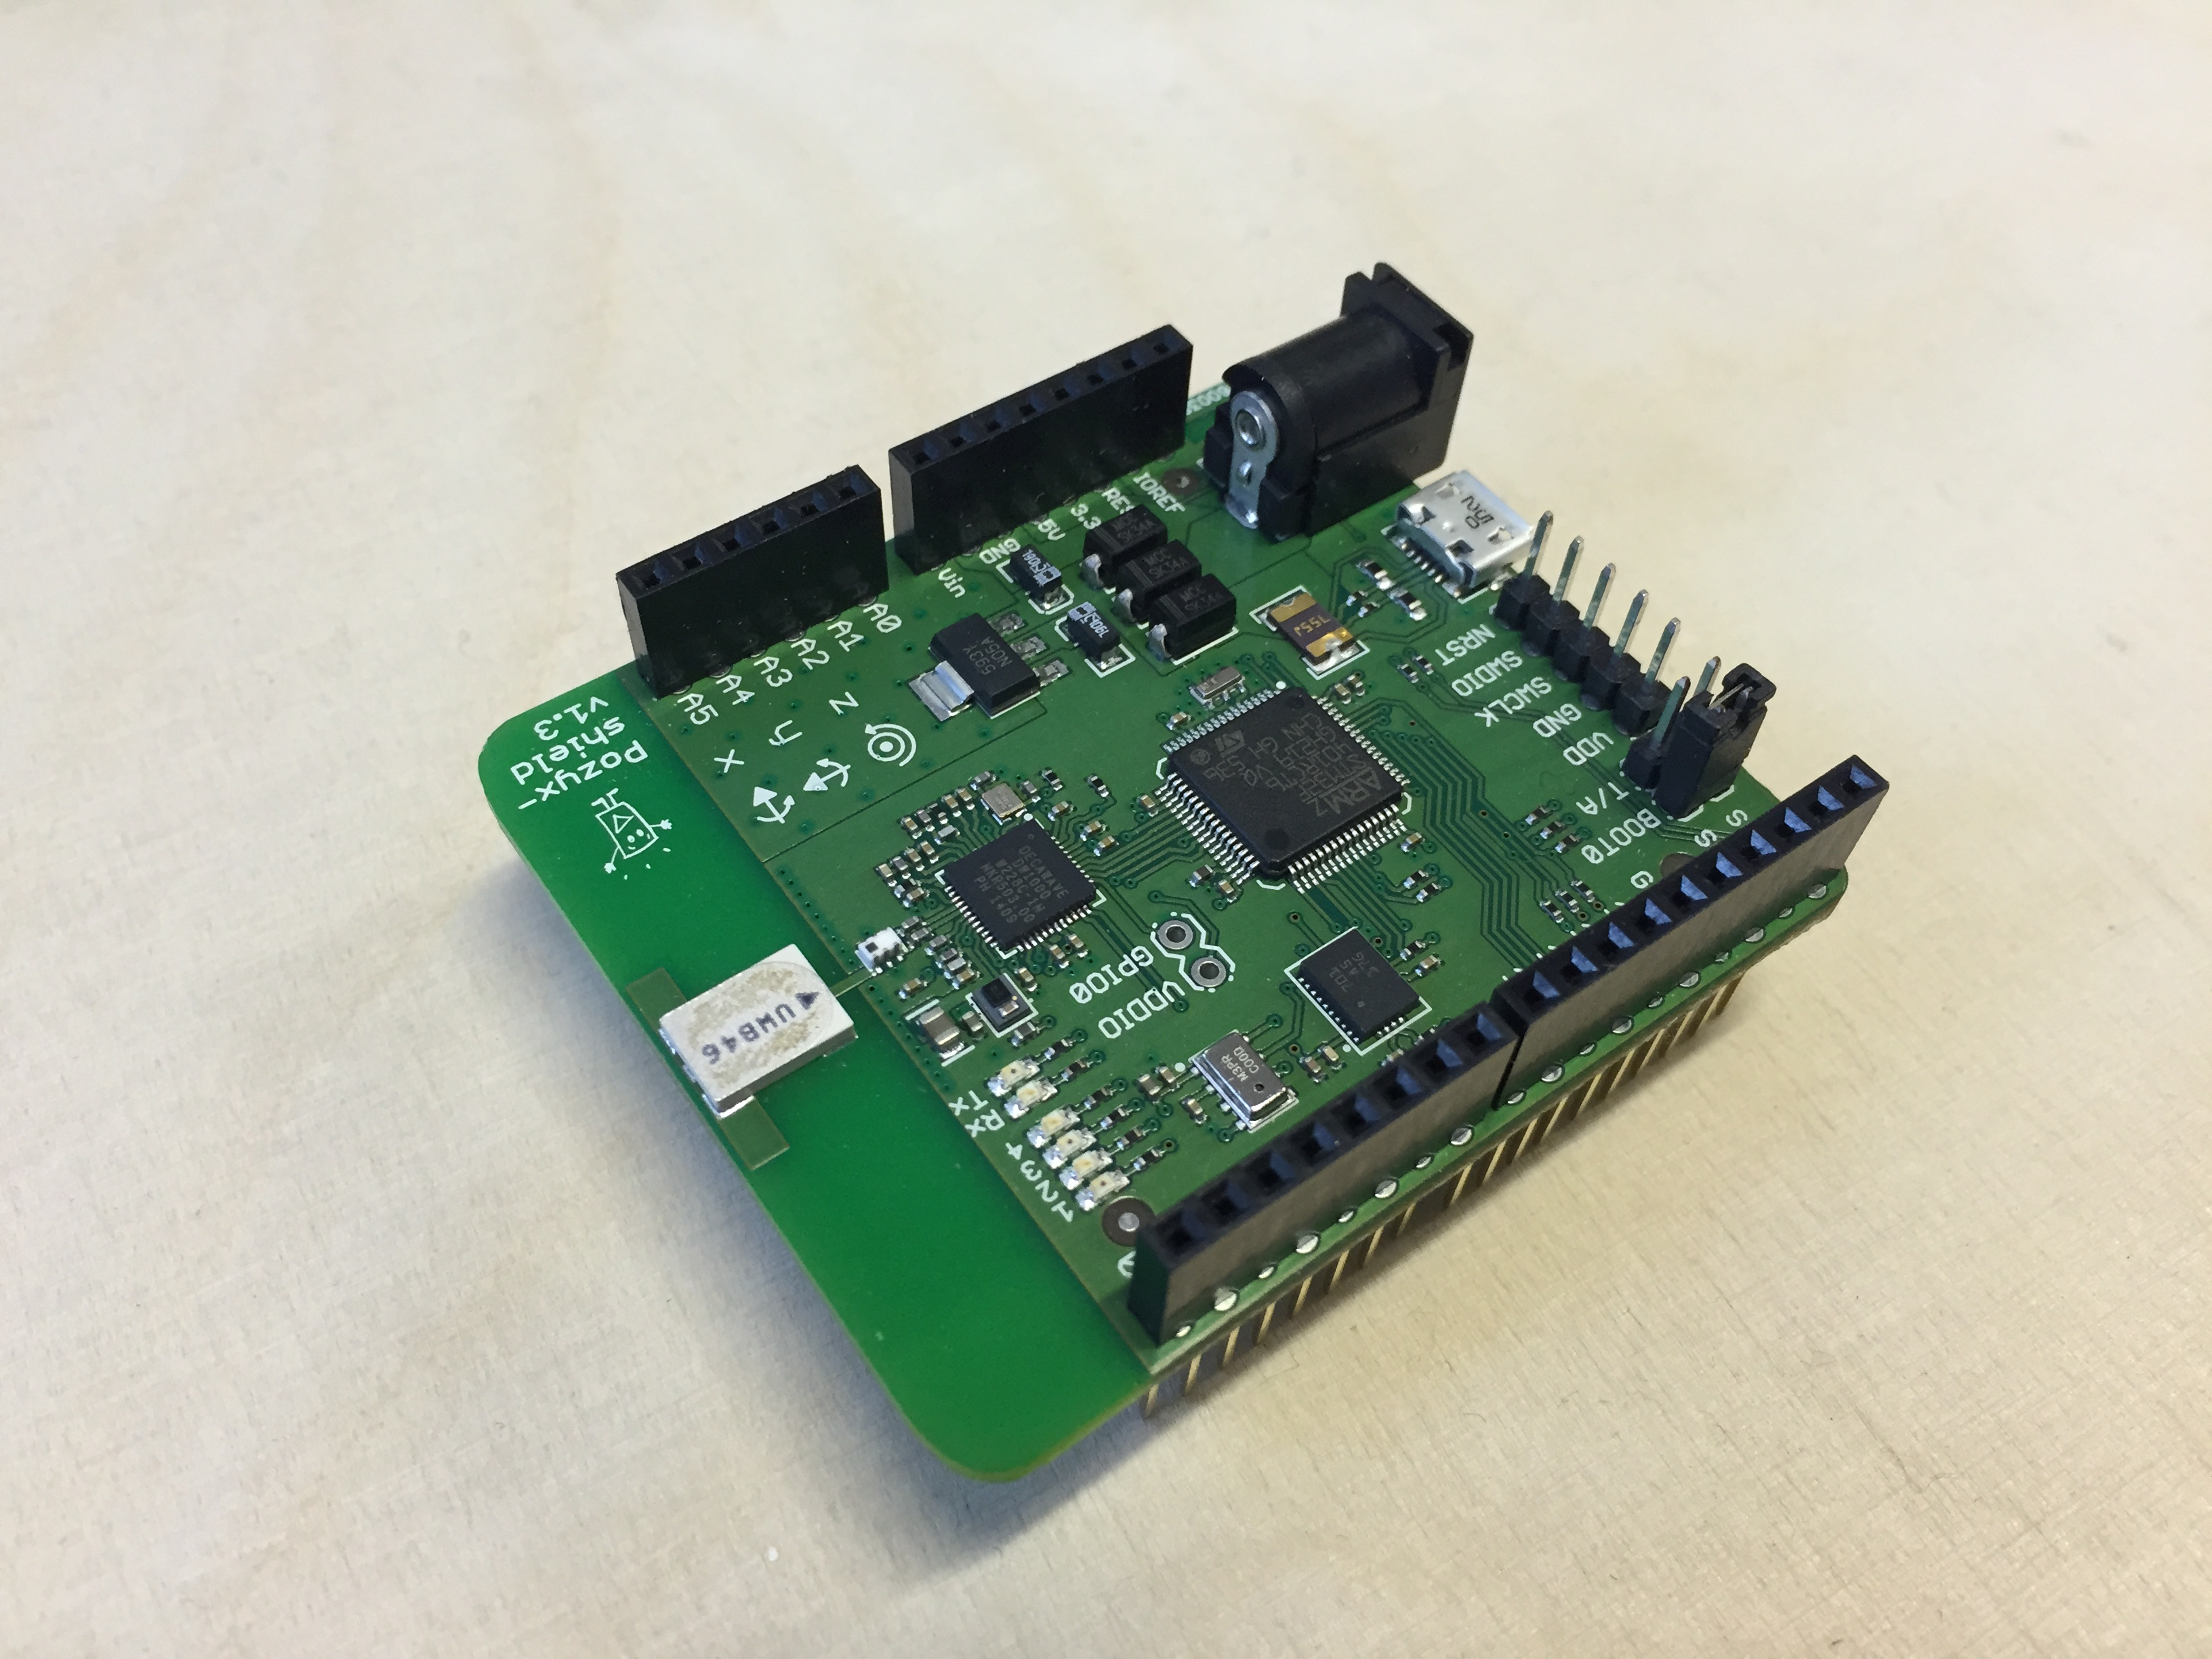
\includegraphics[width=0.5\linewidth]{../fig/pozyx_tag}
	\caption{Picture of Pozyx tag/anchor (Photo: \url{http://pozyx.io})}
	\label{fig:pozyx_tag}
\end{figure}


\subsection{Arduino}
In a very early stage we discussed creating our own tracking devices using Arduino boards and soldering and connecting Bluetooth-antennas to them to create a Bluetooth-transmitter.
We soon discovered that this was a field none of us had any experience with, and it would probably have taken far too much time to develop this solution.
The probability of us creating a product, in such a short time, that would be comparable to the available off-the-shelf products is also low.

\subsection{Estimote}
Another popular beacon manufacturer is Estimote who produces a variety of BLE beacons \citep{EstimoteInc.2018}.
Together with their beacons Estimote also supplies a Software Development Kit (SDK) which theoretically should make it easy to interact with the beacons.
But when we started our planning and development we were warned against using their beacons and SDK because of the many bugs and instabilities in the SDK, and they even dropped support for their old version of it to create a new one from scratch \citep{Saetre2017}.


\onlyinsubfile{\bibliographystyle{chicago}}
\onlyinsubfile{\bibliography{../library}}
\end{document}
